\documentclass[a4paper, 11pt, oneside]{article}

\newcommand{\plogo}{\fbox{$\mathcal{PL}$}} 
\usepackage{amsmath}
\usepackage[utf8]{inputenc} 
\usepackage[T1]{fontenc} 
\usepackage{enumitem}
\usepackage{graphicx}
\usepackage{graphicx}
\usepackage{supertabular}
\usepackage[spanish]{babel}
\graphicspath{{Imagenes/}}

\begin{document} 

\begin{titlepage} 

	\centering 
	
	\scshape 
	
	\vspace*{\baselineskip} 
	
	
	
	\rule{\textwidth}{1.6pt}\vspace*{-\baselineskip}\vspace*{2pt} 
	\rule{\textwidth}{0.4pt} 
	
	\vspace{0.75\baselineskip} 
	
	{\LARGE Resumen 10: Estructura de Directorios}	
	\vspace{0.75\baselineskip} 
	
	\rule{\textwidth}{0.4pt}\vspace*{-\baselineskip}\vspace{3.2pt}
	\rule{\textwidth}{1.6pt} 
	
	\vspace{2\baselineskip} 
	

	ADMINISTRACIÓN DE SISTEMAS UNIX/LINUX
	
	\vspace*{3\baselineskip} 
	
	
	
	Alumna:
	
	\vspace{0.5\baselineskip} 
	
	{\scshape\Large Karla Adriana Esquivel Guzmán \\} 
	\vspace{0.5\baselineskip} 
	\vfill
	
\includegraphics{unam.jpg}
	
	\textit{UNIVERSIDAD NACIONAL AUTONOMA DE MEXICO} 
	
	\vfill
	
	
	
	
	\vspace{0.3\baselineskip} 
	
	11/Febrero/2019 
	
	 

\end{titlepage}

Puesto que se hablo de dispositivos ``montados'' se utilizaba \textbf{ls /\ mnt/\ } para montar particiones, sólo se hablo de ese comando sin mayor profundidad, para ver los directorios utilizamos \textbf{cd /\ } y después el comando \textbf{ls}.
\begin{center}
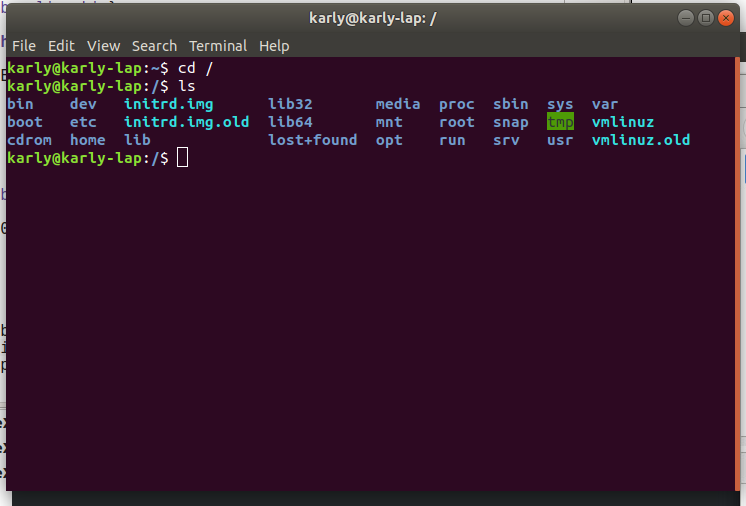
\includegraphics[scale=0.35]{11102.png} 
\end{center}

Con \textbf{df -lh} podemos ver lo que está ``montado'' como los dispositivos de almacenamiento.

\begin{center}
 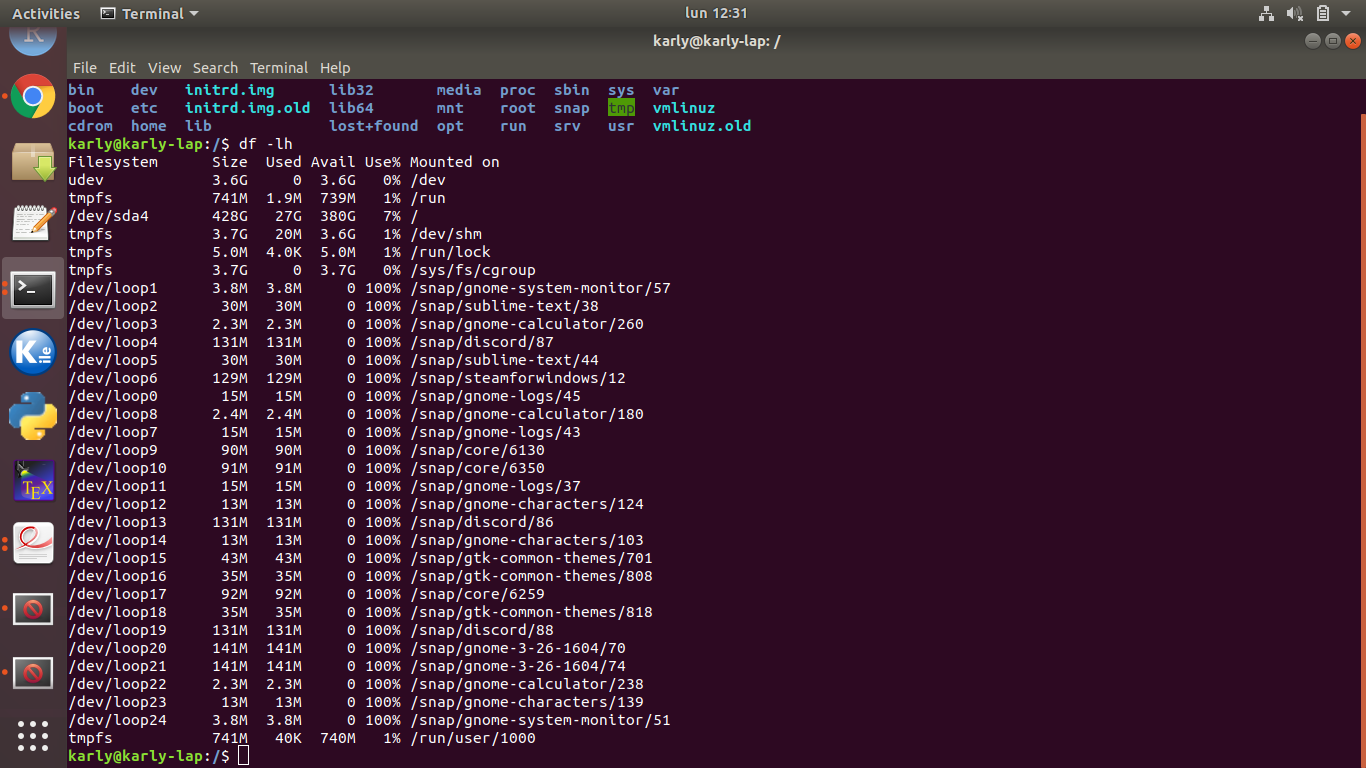
\includegraphics[scale=0.20]{21102.png}
\end{center}


Serial ATA: formato en que están transferidos los datos.
\begin{center}
 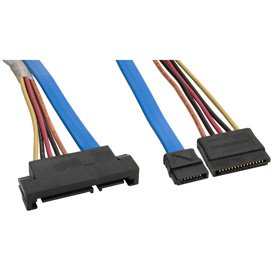
\includegraphics[scale=0.30]{31102.jpg}
\end{center}

Se habló de la interfaz ``SCSI'' sirve para la transferencia de datos entre distintos dispositivos del bus de la computadora. Hay 3 tipo de SCSI:
\begin{itemize}
 \item SCSI 1 con bus de 8 bits con velocidad de 5MB/s.
 \item SCSI 2 con bus de 8 bits pero velocidad de transmisión de 10MB/s.
 \item SCSI 3 con bus de 16 bits y velocidad de 20MBps/s.
\end{itemize}

\newpage
después ocupamos el comando \textbf{ls boot/\ } para ver archivo de configuración del grub. Si borras algo que no se debe inmediatamente apagas el equipo e inicias con un disco de recuperación.

La tarea que el profesor dejó para el viernes es :
\textbf{Hacer un mapa mental o algo para estudiar, para poder pasar el viernes}
\begin{center}
 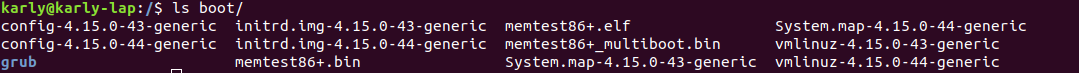
\includegraphics[scale=0.30]{41102}
\end{center}

\end{document}
